%%%%%%%%%%%%%%%%%%%%%%%%%%%%%%%%%%%%%%%%%
% Beamer Presentation
% LaTeX Template
% Version 1.0 (10/11/12)
%
% This template has been downloaded from:
% http://www.LaTeXTemplates.com
%
% License:
% CC BY-NC-SA 3.0 (http://creativecommons.org/licenses/by-nc-sa/3.0/)
%
%%%%%%%%%%%%%%%%%%%%%%%%%%%%%%%%%%%%%%%%%

% ----------------------------------------------------------------------------------------
% PACKAGES AND THEMES
% ----------------------------------------------------------------------------------------

\documentclass{beamer}

\mode<presentation> {

  % The Beamer class comes with a number of default slide themes
  % which change the colors and layouts of slides. Below this is a list
  % of all the themes, uncomment each in turn to see what they look like.

  % \usetheme{default}
  % \usetheme{AnnArbor}
  % \usetheme{Antibes}
  % \usetheme{Bergen}
  % \usetheme{Berkeley}
  % \usetheme{Berlin}
  % \usetheme{Boadilla}
  % \usetheme{CambridgeUS}
  % \usetheme{Copenhagen}
  % \usetheme{Darmstadt}
  % \usetheme{Dresden}
  % \usetheme{Frankfurt}
  % \usetheme{Goettingen}
  % \usetheme{Hannover}
  % \usetheme{Ilmenau}
  % \usetheme{JuanLesPins}
  % \usetheme{Luebeck}
  \usetheme{Madrid}
  % \usetheme{Malmoe}
  % \usetheme{Marburg}
  % \usetheme{Montpellier}
  % \usetheme{PaloAlto}
  % \usetheme{Pittsburgh}
  % \usetheme{Rochester}
  % \usetheme{Singapore}
  % \usetheme{Szeged}
  % \usetheme{Warsaw}

  % As well as themes, the Beamer class has a number of color themes
  % for any slide theme. Uncomment each of these in turn to see how it
  % changes the colors of your current slide theme.

  % \usecolortheme{albatross}
  % \usecolortheme{beaver}
  % \usecolortheme{beetle}
  % \usecolortheme{crane}
  % \usecolortheme{dolphin}
  % \usecolortheme{dove}
  % \usecolortheme{fly}
  % \usecolortheme{lily}
  % \usecolortheme{orchid}
  % \usecolortheme{rose}
  % \usecolortheme{seagull}
  % \usecolortheme{seahorse}
  % \usecolortheme{whale}
  % \usecolortheme{wolverine}

  % \setbeamertemplate{footline} % To remove the footer line in all slides uncomment this line
  % \setbeamertemplate{footline}[page number] % To replace the footer line in all slides with a simple slide count uncomment this line

  % \setbeamertemplate{navigation symbols}{} % To remove the navigation symbols from the bottom of all slides uncomment this line
}

\usepackage{graphicx} % Allows including images
\usepackage{booktabs} % Allows the use of \toprule, \midrule and \bottomrule in tables
\usepackage{multirow}
\usepackage{adjustbox}
\usepackage{array}
\usepackage{tikz}
\usepackage{soul}
\usetikzlibrary{shapes.geometric, arrows, positioning, fit}
\usepackage[latin1]{inputenc}
\newcommand{\xmark}{\textcolor{red}{\text{\sffamily X}}}
\newcommand{\cmark}{\textcolor{green}{\checkmark}}
\newcommand{\tr}{\text{tr}}
\newcommand{\E}{\textbf{E}}
\newcommand{\diag}{\text{diag}}
\newcommand{\argmax}{\text{argmax}}
\newcommand{\argmin}{\text{argmin}}
\newcommand{\Cov}{\text{Cov}}
\newcommand{\Var}{\text{Var}}
\newcommand{\Vol}{\text{Vol}}
\newcommand{\bx}{\boldsymbol{x}}
\newcommand{\by}{\boldsymbol{y}}
\newcommand{\bX}{\boldsymbol{X}}
\newcommand{\bY}{\boldsymbol{Y}}
\sethlcolor{gray}
\makeatletter
\newcommand\SoulColor{%
  \let\set@color\beamerorig@set@color
  \let\reset@color\beamerorig@reset@color}
\makeatother
\definecolor{color1}{RGB}{128,0,0}
\definecolor{color2}{RGB}{0,128,0}
\definecolor{color3}{RGB}{0,0,128}
\definecolor{color4}{RGB}{70,13,128}

\newcommand\independent{\protect\mathpalette{\protect\independenT}{\perp}}
\def\independenT#1#2{\mathrel{\rlap{$#1#2$}\mkern2mu{#1#2}}}

% tikz stufff


% ----------------------------------------------------------------------------------------
% TITLE PAGE
% ----------------------------------------------------------------------------------------


\title[Informal]{Causal Inference and Invariance}

\author[Zhao and Zheng]{Qingyuan Zhao and Charles Zheng}
\institute[Stanford]
{Stanford University}
\date{\today}

\begin{document}

\begin{frame}
  \titlepage
  (Part 2/2)
\end{frame}

\begin{frame}
  \frametitle{From Last Week: Causal Graph}
  Causal relationships in a system represented by a graph.  The graph tells you:
  \begin{itemize}
  \item[I.] which variables are affected by an intervention.
  \item[II.] what conditional independence relationships exist in the joint distribution (\emph{d-separation}.)
  \item[III.] which sets of predictors and responses will have ``invariant'' optimal predictive rules.
  \end{itemize}

  This talk is restricted to directed acyclic graph (DAG), i.e.\ no feedback!
\end{frame}

\begin{frame}
  \frametitle{From Last Week: Three \emph{Causal} Questions}
  \begin{itemize}
  \item Given a number of variables, which pairs are causally related?
    \begin{itemize}
    \item Infer the \emph{graph}.
    \end{itemize}
  \item Given a number of variables and a fixed $Y$, which variables
    causally affect $Y$?
    \begin{itemize}
    \item Infer the \emph{invariance set}.
    \end{itemize}
  \item Given a fixed $X$ and a fixed $Y$, what is the causal effect of
    $X$ on $Y$?
    \begin{itemize}
    \item Infer the \emph{causal effect}.
    \end{itemize}
  \end{itemize}

  \begin{center}
    Why different languages? Convenience!
  \end{center}

\end{frame}

\section{Overview of Previous methods}
\label{sec:previous-methods}

\begin{frame}
  \sectionpage
\end{frame}

\begin{frame}
  \frametitle{Known Causal Structure}
  \begin{center}
    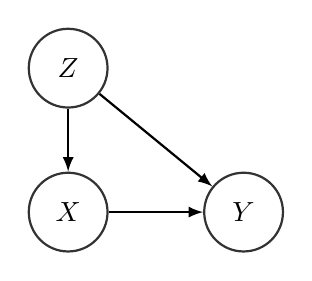
\begin{tikzpicture}[node distance = 8mm and 12mm]
      \tikzstyle{main} = [circle, minimum size = 10mm, thick, draw = black!80]
      \tikzstyle{connect} = [-latex, thick]
      \node[main] (x) {$X$};
      \node[main, right=of x] (y) {$Y$};
      \node[main, above=of x] (z) {$Z$};
      \path (x) edge [connect] (y) (z) edge [connect] (y) (z) edge [connect] (x);
    \end{tikzpicture}
  \end{center}
  For example, suppose we want to estimate the causal effect of $X$ on $Y$ with
  known confounders $Z$.
  \begin{itemize}
  \item Graphical approach: the backdoor formula
    \vspace{-0.5em}
    \[
    \begin{split}
      \mathrm{P}(y|do(x)) = \sum_z \mathrm{P}(y|x, z) \mathrm{P}(z).
    \end{split}
    \]
    \vspace{-2em}
  \item Functional approach: outcome regression $Y \sim X + Z$.
  \item Potential outcome approach: estimate the propensity score.
  \end{itemize}
\end{frame}

\begin{frame}

  \frametitle{Unknown Causal Structure}
  Conventional approach:
  \begin{enumerate}
  \item Estimate the Markov equivalence class of causal graphs via conditional
    independence relationships.
  \item Infer or bound the identifiable causal effects.
  \end{enumerate}

  \vspace{1em}

  More recent approach: impose additional functional/distributional
  assumptions to the structural equation model: for any variable $Y$,
  \[
  Y = f(\mathrm{parents}(Y);\epsilon_Y).
  \]

\end{frame}

\begin{frame}
  \frametitle{How should we think about the assumptions?}
  \begin{center}
    One thing for sure: They are no monsters!
  \end{center}
  \vspace{12em}
  \begin{figure}
    \centering
    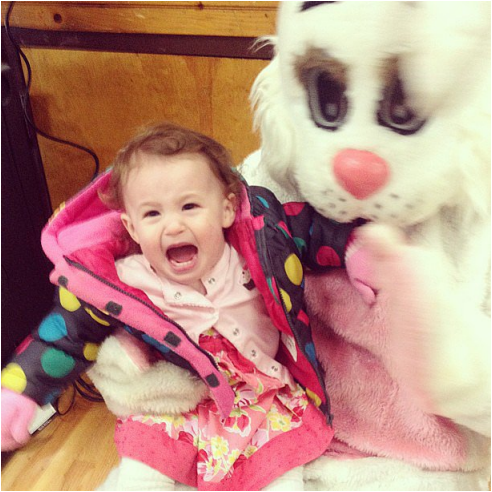
\includegraphics[scale = 0.0045, angle=180]{../images/no_monster.jpg}
  \end{figure}

\end{frame}

\begin{frame}
  \frametitle{How should we think about the assumptions?}
  \begin{itemize}
  \item In statistics we make assumptions all the
    time: parametric, independence, function form, etc.
    \begin{itemize}
    \item George Box: ``All models are wrong but some are useful''.
    \end{itemize}
  \item To infer causation, we need to make different kinds of
    assumptions.
    \begin{itemize}
    \item Problem statement: Can what we learned from this environment
      be generalized to another environment?
    \item The ancient wisdom: ``Correlation does not imply
      causation'' (observational $\not \Rightarrow$ interventional).
    \item Causal assumptions: causal graph, structural equation model,
      or invariant prediction.
    \end{itemize}
  \end{itemize}

  \begin{center}
    What if we are willing to make both kinds of assumptions?
  \end{center}
\end{frame}

\section{Invariance}

\begin{frame}
  \sectionpage
\end{frame}

\begin{frame}
  \frametitle{Assumed invariance}
  Focus: Given a number of variables and a fixed $Y$, which variables
  causally affect $Y$?

  Data: i.i.d.\ samples of $(X^e,Y^e)$ from different environments $e
  \in \mathcal{E}$.

  \begin{block}{Assumption (Invariant prediction)}
    There exists a vector of coefficients $\gamma^{*}$ with support
    $S^{*}$ such that for all $e \in \mathcal{E}$, $X^e$ has an arbitrary
    distribution and
    \[
    Y^e = \mu + X^e \gamma^{*} + \epsilon^e,~\epsilon^e \sim
    F_{\epsilon},~\epsilon^e \independent X^e_{S^{*}}.
    \]
  \end{block}
  Important:
  \begin{itemize}
  \item $F_{\epsilon}$ does not depend on $e$.
  \item $\epsilon$ is always independent of $X$.
  \end{itemize}

  This is essentially a single structural equation with
  $\mathrm{parents}(Y) = S^{*}$.
\end{frame}

\begin{frame}
  \frametitle{Building block}
  Testing the null hypothesis that $(\gamma,S)$
  satisfies the assumption.
  \[
  \begin{split}
    H_{0,\gamma,S}(\mathcal{E}):~&\gamma_k = 0~\mathrm{if}~k \in S,~and~
    \exists F_{\epsilon} \mathrm{~such~that~for~all~} e \in \mathcal{E}, \\
    &Y^e = X^e \gamma + \epsilon^e,~\epsilon^e \sim F_{\epsilon},~ \epsilon^e \independent X^e_{S}.\\
    H_{0,S}(\mathcal{E}):~&\exists \gamma \mathrm{~such~that~}
    H_{0,\gamma,S}(\mathcal{E}) \mathrm{~is~true}.
  \end{split}
  \]

  \begin{alertblock}{Difficulty}
    \begin{center}
      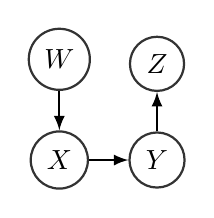
\begin{tikzpicture}[node distance = 5mm and 5mm]
        \tikzstyle{main} = [circle, minimum size = 3mm, thick, draw = black!80]
        \tikzstyle{connect} = [-latex, thick]
        \node[main] (x) {$X$};
        \node[main, right=of x] (y) {$Y$};
        \node[main, above=of x] (w) {$W$};
        \node[main, above=of y] (z) {$Z$};
        \path (x) edge [connect] (y) (w) edge [connect] (x) (y) edge [connect] (z);
      \end{tikzpicture} \qquad
      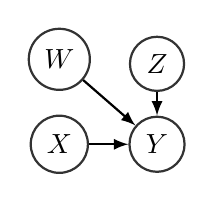
\begin{tikzpicture}[node distance = 3mm and 5mm]
        \tikzstyle{main} = [circle, minimum size = 3mm, thick, draw = black!80]
        \tikzstyle{connect} = [-latex, thick]
        \node[main] (x) {$X$};
        \node[main, right=of x] (y) {$Y$};
        \node[main, above=of x] (w) {$W$};
        \node[main, above=of y] (z) {$Z$};
        \path (x) edge [connect] (y) (w) edge [connect] (y) (z) edge [connect] (y);
      \end{tikzpicture}
    \end{center}

    Statistically, we may end up accepting both $Y^e = X ^e+ \epsilon^e$ and $Y^e = X ^e + 0.01
    W^e + 0.01 Z^e + \epsilon^e$, for both causal structures.
  \end{alertblock}

\end{frame}

\begin{frame}
  \frametitle{Generic procedure}
  \begin{exampleblock}{}
    \begin{enumerate}
    \item For each $S \subseteq \{1,\dotsc,p\}$, test
      $H_{0,S}(\mathcal{E})$ at level $\alpha$.
    \item Set $\hat{S}(\mathcal{E}) =
      \underset{S:H_{0,S}(\mathcal{E})\mathrm{~not~rejected}}{\bigcap}
      S$.
    \item For the confidence sets, set $\hat{\Gamma}(\mathcal{E}) =
      \underset{S \subseteq \{1,\dotsc,p\}}{\bigcup}
      \hat{\Gamma}_S(\mathcal{E})$, where
      \[
      \hat{\Gamma}_S(\mathcal{E}) =
      \begin{cases}
        \emptyset &
        H_{0,S}(\mathcal{E})\mathrm{~is~rejected~at~level~}\alpha, \\
        \hat{S} & \mathrm{otherwise}.
      \end{cases}
      \]
      $\hat{C}(S)$ is a $(1-\alpha)$-confidence set for $\gamma$ obtained by
      pooling the data.
    \end{enumerate}
  \end{exampleblock}

  \begin{block}{Theorem (Peters et al.)} \centering
    $\mathrm{P}(\hat{S}(\mathcal{E}) \subseteq S^{*}) \ge 1-\alpha,~
    \mathrm{P}(\gamma^{*} \in \hat{\Gamma}(\mathcal{E})) \ge 1 - 2\alpha$.
  \end{block}
\end{frame}

\begin{frame}
  \frametitle{The Statistical Challenge}
  Depending on the modeling assumption, this hypothesis can be:
\[
\begin{split}
    H_{0,S,\mathrm{lin}}(\mathcal{E}):~&\exists \gamma \mathrm{~s.t.~} \gamma_k =
    0~\mathrm{if}~k \in S, and \\ ~&
    \exists F_{\epsilon} \mathrm{~s.t.~} Y^e = X^e \gamma +
    \epsilon^e,~\epsilon^e \sim F_{\epsilon},~ \epsilon^e \independent
    X^e_{S},~\forall e \in \mathcal{E}. \\
    H_{0,S,\mathrm{lin\textrm{-}gauss}}(\mathcal{E}):~&
    H_{0,S,\mathrm{lin}}(\mathcal{E}) \mathrm{~and~} F_{\epsilon} = \mathrm{N}(0,\sigma^2). \\
    H_{0,S,\mathrm{nonlin}}(\mathcal{E}):~&\exists g(X_S,\epsilon),~F_{\epsilon} \mathrm{~s.t.~}
    Y^e = g(X_S^e, \epsilon^e),~\epsilon^e\ldots.\\
    H_{0,S,\mathrm{additive}}(\mathcal{E}):~&H_{0,S,\mathrm{nonlin}}(\mathcal{E})
    \mathrm{~and~} g(X_S,\epsilon) \mathrm{~is~additive}.\\
    H_{0,S,\mathrm{hidden}}(\mathcal{E}):~&\epsilon^e \sim
    F_{\epsilon}, ~ \forall e \in
    \mathcal{E},~\mathrm{but}~F_{\epsilon}\mathrm{~can~have~nonzero~mean}.\\
\end{split}
\]

  \begin{exampleblock}{How to test $H_{0,S}(\mathcal{E})$?}
  Peters et al.\ give concrete proposals for $H_{0,S,\mathrm{lin\textrm{-}gauss}}$ and
  $H_{0,S,\mathrm{lin\textrm{-}gauss\textrm{-}hidden}}$. They are implemented in their
  \texttt{InvariantCausalPrediction} package.
  \end{exampleblock}

\end{frame}

\begin{frame}
  \frametitle{Robustness of the invariance approach}
  In Meinshausen's talk: we don't make false discoveries, even under a
  misspecified model!

  Truth (at least what we believe in):

  \begin{center}
  \begin{tabular}{|c|c|}
    \hline
    Things can go wrong & ICP's behavior \\
    \hline
    Intervene on $Y$ (or a missing cause) &
    $\underset{\emptyset}{\bigcap}$ \\
    \hline
    Non-linear, non-additive &
    $\underset{\emptyset}{\bigcap}$ \\
    \hline
    Not enough interventions &
    False positives \\
    \hline
    Small sample size &
    $\emptyset$ \\
    \hline
    Left out a confounder & $\emptyset$ \\
    \hline
    Left out an unconfounding predictor & okay \\
    \hline
  \end{tabular}
  \end{center}
\end{frame}

\begin{frame}
  \frametitle{Splitting purely observational data}
  A big bonus: we can ``create'' an environment by conditioning on a
  variable $U$ that we know precedes $Y$. This is valid because
\[
Y|X_{S^{*}} ~\overset{d}{=}~ Y|X_{S^{*}},U=u.
\]
  Note: this statement is true only in the region that both
  conditional distributions are well defined.

  \begin{exampleblock}{Creating environment by instrumental variable}
    \begin{center}
        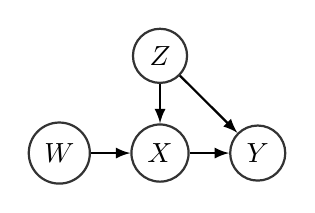
\begin{tikzpicture}[node distance = 5mm and 5mm]
        \tikzstyle{main} = [circle, minimum size = 3mm, thick, draw = black!80]
        \tikzstyle{connect} = [-latex, thick]
        \node[main] (x) {$X$};
        \node[main, right=of x] (y) {$Y$};
        \node[main, left=of x] (w) {$W$};
        \node[main, above=of x] (z) {$Z$};
        \path (x) edge [connect] (y) (w) edge [connect] (x) (z) edge
        [connect] (x) (z) edge [connect] (y);
      \end{tikzpicture}
    \end{center}
    If there is a hidden confounder $Z$, we can condition on the
    instrumental variable $W$.
  \end{exampleblock}
\end{frame}

\begin{frame}
  \frametitle{Back to the three causal questions}
  Can ICP help to answer the other two questions?
  \begin{block}{Infer the graph}
    We can run ICP for every node with caution. Returns a partially
    identified graph.
  \end{block}

  \begin{block}{Infer the causal effect of $X$ on $Y$}
    Two options:
    \begin{itemize}
    \item Treat $X$ as the target variable: \emph{propensity score}.
    \item Treat $Y$ as the target variable: \emph{outcome regression}.
    \end{itemize}
    Okay if $\hat{S}$ itself is invariant. Otherwise ICP may miss important causes, resulting
    in biased causal effect estimate.

    Idea: maybe we can just use (many) ``minimal'' $S$.
  \end{block}
\end{frame}

\end{document}
%%% Local Variables:
%%% mode: latex
%%% TeX-master: t
%%% End:
